%% Diagram to motivate building weight matrices
\documentclass[tikz]{standalone}
\usepackage[sfdefault]{cabin}

\renewcommand{\vec}{\mathbf}

\usetikzlibrary{arrows.meta, bending, decorations.pathreplacing, positioning, shapes}
\tikzstyle{every picture}+=[remember picture]
\tikzset{
    neuron/.style = {
      fill=gray, circle, text width=5pt, text height=5pt, inner sep=0,
      draw=black!65!white, ultra thick,
    },
    synapse/.style = {
      thick, black!75!white, shorten >= 2.5pt, arrows={-Triangle[]},
    },
    synaptic weight/.style = {
      very thick, draw, fill=white,
    },
    weak synapse/.style = {
      synapse, black!25!white,
    },
    vector/.style = {
      thick, arrows={-Triangle[]},
    },
}

\begin{document}
  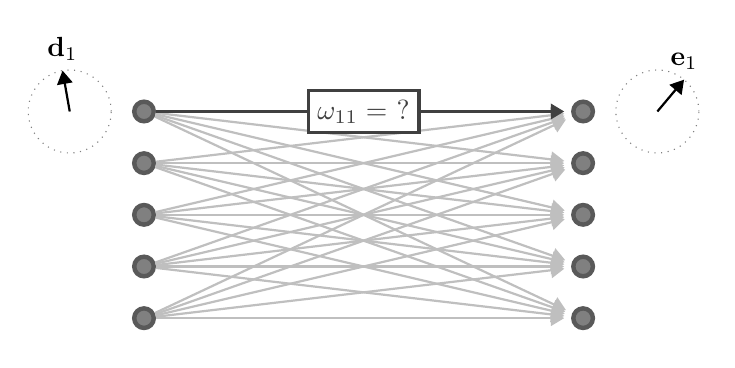
\begin{tikzpicture}
    %% Draw two populations of neurons, connect all but the first pair together
    \matrix [column sep=15em, row sep=1em] {
      \node [neuron] (n11) {}; & \node [neuron] (n12) {}; \\
      \node [neuron] (n21) {}; & \node [neuron] (n22) {}; \\
      \node [neuron] (n31) {}; & \node [neuron] (n32) {}; \\
      \node [neuron] (n41) {}; & \node [neuron] (n42) {}; \\
      \node [neuron] (n51) {}; & \node [neuron] (n52) {}; \\
    };

    %% Connect all but the first pair
    \foreach \i in {2,...,5}{%
      \foreach \j in {1,...,5}{%
        \draw [weak synapse] (n\i1) -- (n\j2);
      }
    }
    \foreach \j in {2,...,5}{%
      \draw [weak synapse] (n11) -- (n\j2);
    }

    %% Connect the first pair
    \draw [synapse] (n11) -- (n12) node [midway, synaptic weight] {$\mathbf{\omega}_{11} = $ ?};

    %% Draw the decoding and encoding vectors
    \draw [black!50!white, dotted] ([xshift=-2.25em] n11.west) circle (1.5em);
    \draw [vector] ([xshift=-2.25em] n11.west) -- ++(100:1.5em) node [above] {$\vec{d}_{1}$};
    \draw [black!50!white, dotted] ([xshift=+2.25em] n12.east) circle (1.5em);
    \draw [vector] ([xshift=+2.25em] n12.east) -- ++(50:1.5em) node [above] {$\vec{e}_{1}$};
  \end{tikzpicture}
\end{document}
